\documentclass{article}

\usepackage[utf8]{inputenc}
\usepackage[T1]{fontenc}
\usepackage[english,francais]{babel}
\usepackage{textcomp}
\usepackage{amsmath,amssymb}
\usepackage{lmodern}
\usepackage[a4paper]{geometry}
\usepackage{graphicx}
\usepackage{xcolor}
\usepackage{microtype}
\usepackage{lipsum}
\usepackage{moreverb}
\usepackage{hyperref}
\hypersetup{pdfstartview=XYZ}

\title{Compte rendu de \og Ghost Legs\fg{}}
\author{Lilian Hiault}
\date{4 avril 2019}

\begin{document}

\maketitle

\tableofcontents

\section*{Introduction}
\og Ghost Legs\fg{} est un problème posé par java\_coffee\_cup sur CodingGames (\url{https://www.codingame.com/training/easy/ghost-legs}). Le but est de créer un programme capable de retrouver un caractère associé à un autre en suivant des lignes. Il faut suivre les lignes verticales et de changer de branche dès qu'une ligne horizontale se présente. Comme on peut le voir dans la figure \ref{exGhostLegs} page \pageref{exGhostLegs}.

\begin{figure}[h]
  \centerline{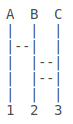
\includegraphics{ex_ghost_legs.png}}
  \caption{Exemple : ici on associe A2, B1, C3}\label{exGhostLegs}
\end{figure}

\section{Comment stocker les données ?}

Mon programme demande d'abord à l'utilisateur d'entrer la largeur et la hauteur du diagramme qu'il va saisir.

\begin{boxedverbatim}
int main()
{
    int L = 0;
    int H = 0;
    //Entrée de la largeur et de la hauteur
    scanf("%d%d", &L, &H);
    fgetc(stdin);
\end{boxedverbatim}
    
\\ \\Lorsque l'utilisateur rentre ligne par ligne le diagramme, il faut le garder afin de l'exploiter. J'ai choisis de stocker chaque ligne dans une ligne d'un tableau.
\\

\begin{boxedverbatim}
  char ** diagramme = (char **) malloc(L*sizeof(char*));
  // On crée un tableau contenant des chaînes de caractères
    int i;
    for(i=0; i<H; i++)
    {
      diagramme[i]=(char *) malloc(L*sizeof(char));
      // A chaque entrée de l'utilisateur (une par itération de la boucle)
      //on crée un second tableau dans chaque case du premier tableau pour
      //qu'il soit en 2 dimensions
      fgets(diagramme[i], 1025, stdin);
      // Dans chaque case on va y placer un caractère
    }
\end{boxedverbatim}

\\\`A ce moment on à donc un tableau en 2 dimensions de pointeurs qui pointent vers des tableaux de caractères? Chaque ligne entrée est stocké dans une ligne du tableau avec chaque caractère séparé dans une case.
\\
La première version de mon programme était assez différente de celle-ci. J'avais fais appel à deux fonctions pour avoir le même résultat. Tout d'abord Une fonction qui créait le tableau en 2 dimensions en entier puis une deuxième qui pour chaque ligne saisie, séparait les caractères pour les insérer dans le tableau? Toutefois cette solution était plus complexes, plus longues et a donc facilité les erreurs.

\section{\`A la recherche d'une solution}

Une fois que tout est stocké dans mon tableau il faut le parcourir afin de trouver la bonne association de caractères.

\begin{boxedverbatim}
  void deplacement(char ** diagramme, int H, int L)
{
    int k=0;
    int i,j;
    for (k=0; k<L; k+=3)
    {
        // Une itération pour chaque lettre
        i=1;
        j=k;
        // Les coordonnées du point de départ
        for(i=1; i<H; i++)
        {
            if ((j>1) && (diagramme[i][j-1] == '-'))
            {
              j-=3;
              // Se déplacer à gauche
            }
            else if ((j<L-1) && (diagramme[i][j+1] == '-'))
            {
              j+=3;
              // Se déplacer à droite
            }
          }
        printf("%c%c\n", diagramme[0][k], diagramme[H-1][j]);
        // Afficher le couple de caractères
      }
}
\end{boxedverbatim}

\subsection{Un point de départ}
Cette fois-ci ma première approche ressemblait assez à la version finale. Tout d'abord il nous faut réitérer la recherche pour chaque lettre, or chaque lettre est espacée de deux caractères, je pose donc une boucle pour avec un pas de 3.
Une fois qu'on est à la recherche du couple de caractères on connaît la postition de départ du premier des deux : au niveau de la première ligne et sur la colonne donnée par la boucle.

\subsection{Et surtout un résultat}
La seconde boucle à chaque itération descendre d'une ligne dans le diagramme. On se place à notre point de départ. \`A chaque nouvelle ligne on effectue un test pour savoir s'il y a une ligne horizontale sur les cases voisines. Si c'est le cas, il faut se déplacer en conséquent de 3 cases (car les colonnes sont espacées de deux caractères) d'un côté ou de l'autre. Une fois arrivé à la dernière ligne en suivant le bon chemin, on a le caractère qu'il nous faut.

\begin{boxedverbatim}
  //suite du programme principal
  deplacement(diagramme, H, L);
  //La fonction qui nous permet de trouver les solutions
  free(diagramme);
  //on libère le tableau
  return 0;
}
\end{boxedverbatim}
\\ \\ Il ne nous reste plus qu'à quitter la fonction et libérer le tableau créé.

\section{Ce que j'ai appris}

Ce  programme m'a permis de tester et d'améliorer mes connaisssances en C. J'ai dû recourir à des pointeurs, des chaînes de caractères, etc... Il est également très intéressant de voir qu'il existe de nombreuses façons différentes de concevoir et de résoudre le problèmes. Certains ont préféré utiliser des structures par exemple plutôt que d'utiliser les tableaux de caractères. De plus pour un programme comme celui-ci qui est plus long que ce dont j'avais l'habitude il faut bien renseigner son code afin qu'il soit lisible. C'est un problème que j'ai apprécié résoudre !


\end{document}
